\documentclass[12pt, letterpaper, twoside]{article}
\usepackage[sectionbib,round]{natbib}
\bibliographystyle{apalike}
\usepackage[utf8]{inputenc}
\usepackage{amsmath}
\usepackage{graphicx} %Loading the package
\graphicspath{{figures/}} %Setting the graphicspath
\usepackage{aas_macros} %commom journal
\usepackage{physunits}
\usepackage{times}
\usepackage{import}
\usepackage{hyperref}

\begin{document}

\section{Introduction}


\citet{spectres+17}
\section{Application}
\section{Performance}

\begin{figure}[h]
	\label{fig:perf}
	\centering
	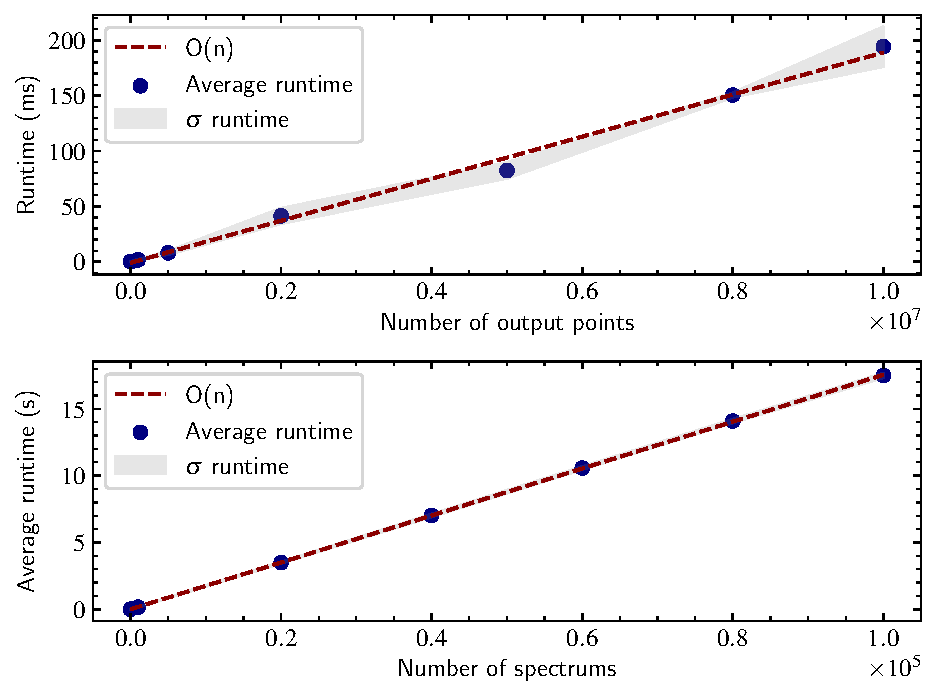
\includegraphics[width = \linewidth]{runtime.pdf}
	\caption{to do}
\end{figure}

\begin{figure}[h]
	\label{fig:perf}
	\centering
	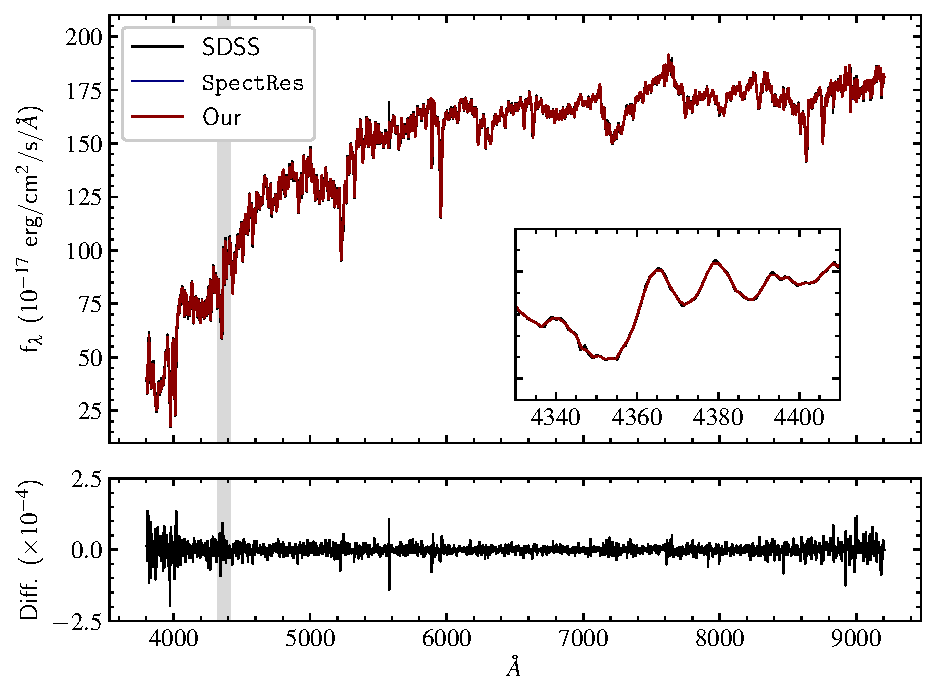
\includegraphics[width = \linewidth]{comparison.pdf}
	\caption{to do}
\end{figure}

\section{Uncertanties propagation}

\bibliography{biblio.bib}

\end{document}
